\runningheader{Oppgave e)}{}{Side \thepage\ av \numpages}
% ********************************************************
% oppgave e) 
% ********************************************************  
\item
  {\bf Numerisk derivasjon som Matlab-funksjon}
\label{oppg:e}
  
  I denne oppgaven skal du lage en egen funksjon av
  bakoverderivasjon. På samme måte som i deloppgave~\ref{oppg:d}) kan
  du velge å  gjøre den frivillige ekstraoppgaven hvor du implementerer alle tre
  metodene og spesifiserer i funksjonskallet hvilken metode du vil
  bruke.

  
  \begin{itemize}
  \item  Koden i skallfilen kaller på
    funksjonen {\tt BakoverDerivasjon} som vist under

\begin{lstlisting}[caption={Kodeutdrag som kaller på funksjonen {\tt BakoverDerivasjon}.},
language= Matlab,  label=kode:bakover2, numbers=none] 
v(1) = 0;   %initialverdi
for ..
    v(k) = BakoverDerivasjon( .., ..);
end
\end{lstlisting}

Med utgangspunkt i bakoverderivasjon gitt som
    \begin{equation}
      \label{eq:1ab}
      v_{k} =\frac{u_{k}-u_{k-1}}{T_s}
    \end{equation}
fullfør koden i skallfilen til funksjonen  
\fbox{\tt  BakoverDerivasjon.m}, gjengitt under.

\begin{lstlisting}[caption={Funksjonen/filen {\tt BakoverDerivasjon.m}.},
language= Matlab,  label=kode:bakover, numbers=none] 
function Sekant = BakoverDerivasjon(FunctionValues, Timestep)
% fyll inn
end
\end{lstlisting}

    Som du ser benytter funksjonen variabelnavn som er matematisk  
    beskrivende, og den skal formuleres uten bruk av indeks {\tt k}. 
\item Kjør koden  og vis at {\tt v(k)} gir samme resultat som 
    {\tt  v\_bakover(k)} i oppgave~\ref{oppg:b}).
  
\end{itemize}

\newpage
\subsubsection*{Generell funksjon for numerisk derivasjon (frivillig)}

For å ha en mer fleksibel derivasjonsrutine skal vi lage en ny
funksjon hvor vi inkluderer et argument som sier noe hvilken
metode som skal brukes.
Et utgangspunkt for dette er funksjonen
{\tt  Derivasjon} vist i kode~\ref{kode:funksjon_num_der}, og denne
finner du igjen i skallfilen \fbox{\tt Derivasjon.m}.

\begin{lstlisting}[caption={Utvidet funksjon for numerisk derivasjon.},
language= Matlab, 
numbers=none,  label=kode:funksjon_num_der]
function Sekant = Derivasjon(FunctionValues, Timestep, options)
arguments
    FunctionValues (1,3) double          % spesifiserer som vektor, 1x3
    Timestep (1,1) double                % spesifiserer som skalar, 1x1
    options.metode (1,:) char = 'Bakover' % metodevalg, default er Bakover
end
    
if strcmp(options.metode,'Forover')
     % fyll inn

elseif strcmp(options.metode,'Bakover')
     % fyll inn

elseif strcmp(options.metode,'Senter')
     % fyll inn

else
    errordlg('Feil metode spesifisert')
    return
end

end
\end{lstlisting}

For å kalle denne funksjonen benyttes syntaksen vist i
kode~\ref{kode:funksjon_num_der_kall} hvor du
ser at de tre siste elementene {\tt  u(k-2:k)}
sendes inn, uansett  metodevalg. Du må derfor passe å plukke ut riktig
element for hver metode i funksjonen.



\begin{lstlisting}[caption={Alternativ bruk av funksjonen {\tt Derivasjon}.},
language= Matlab,  label=kode:funksjon_num_der_kall, numbers=none]
v(k)   = Derivasjon(u(k-2:k), T_s, metode='Bakover');
v(k-1) = Derivasjon(u(k-2:k), T_s, metode='Forover');
v(k-1) = Derivasjon(u(k-2:k), T_s, metode='Senter');
\end{lstlisting}

For å sende inn tre verdier av {\tt u} så kan ikke funksjonen
kalles på før $k{=}3$. Det betyr også at noe må gjøres med
initialverdiene, og dette er vist i skallfilen.

Vis at ved å kjøre koden så får du resultatet vist i figur~\ref{fig:3e_o}. 

    \begin{figure}[H]
      \centering
      \hspace*{0mm}\scalebox{0.5}{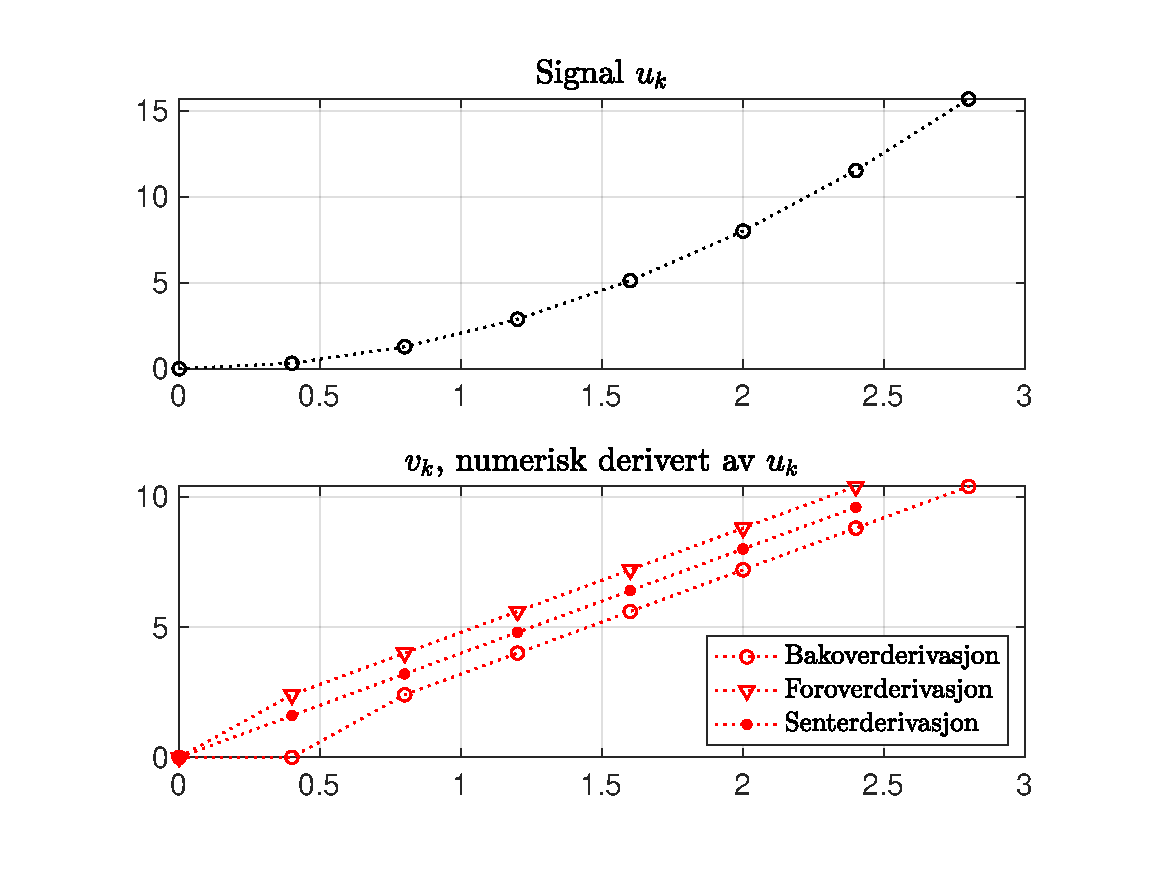
\includegraphics{fig3e_1.pdf}}
      \caption{Resultat av numerisk derivasjon ved bruk av funksjonen
        {\tt Derivasjon}. }
      \label{fig:3e_o}
    \end{figure}
